\documentclass[landscape]{foils}
\usepackage[pdftex]{color}
\usepackage[pdftex]{graphicx}
\usepackage{eso-pic}
\usepackage[top=2cm, bottom=2cm, outer=0cm, inner=0cm]{geometry}
\usepackage{listings}
\usepackage{amsmath}
\usepackage{bold-extra}


\DeclareMathOperator{\sign}{sign}

% colors
\definecolor{DarkRed}{rgb}{0.5,0.0,0.0}
\definecolor{DarkBlue}{rgb}{0.0,0.0,0.35}
\definecolor{DarkGreen}{rgb}{0.0,0.6,0.00}
\definecolor{Orange}{rgb}{0.70,0.30,0.0}
\definecolor{Magenta}{rgb}{0.8,0.0,0.8}
\definecolor{DarkGray}{rgb}{0.3,0.3,0.3}
\definecolor{LightGray}{rgb}{0.9,0.9,0.9}
\definecolor{WhiteGray}{rgb}{0.99,0.99,0.99}
\definecolor{burgundy}{rgb}{0.667,0.110,0.094}
\def\burgundy{\color{burgundy}}
\def\red{\color{red}} 
\def\darkred{\color{DarkRed}} 
\def\blue{\color{DarkBlue}} 
\def\green{\color{DarkGreen}} 
\def\orange{\color{Orange}}
\def\magenta{\color{Magenta}}
\def\black{\color{black}}
\def\gray{\color{DarkGray}}
\def\shade{\color{LightGray}}
\def\hide{\color{WhiteGray}}

% sizes, footer and headers
\textwidth = 26truecm
\textheight = 18truecm
\topmargin =-2 cm
\oddsidemargin -1.5cm
\rightfooter{}
%
\def\indent{\hspace*{1cm}}
\def\prompt{\texttt{\$~}}
\def\prompt{{\footnotesize $\bullet$}~}
\def\exec#1{\indent\prompt\code{#1}}
\def\codeline#1{\indent\code{#1}}
\parindent 0pt

% alias for slides header
\def\Head#1{\foilhead{\burgundy #1 \vskip -1cm} \medskip\hrule\medskip}
\def\head#1{\foilhead{\burgundy #1 \vskip -1cm}}

% aliases for codes, files, namelists, etc.
\def\codecolor{\green}
\def\cardcolor{\orange}
\def\code#1{\texttt{\codecolor #1}}
\def\prog#1{\texttt{\burgundy #1}}
\def\var#1{\texttt{\burgundy #1}}
\def\file#1{\texttt{\green #1}}
\def\cmd#1{\texttt{\green #1}}
\def\nml#1{\texttt{\magenta #1}}
\def\card#1{\texttt{\cardcolor #1}}
\def\flag#1{\texttt{\green #1}}

% aliases for math
\def\vr{\ensuremath{\bm{r}}}
\def\vR{\ensuremath{\bm{R}}}
\def\vk{\ensuremath{\bm{k}}}
\def\vtau{\ensuremath{\bm{\tau}}}


\begin{document}

\blue
\vspace*{0.75cm}
\begin{center}

\includegraphics[width=0.45\textwidth]{../pictures/quantum_ogo_ok-1536x412.png}
\end{center}
~\\
%\vspace*{2cm}
%\MyLogo{~}
\vspace{0.80em}
\begin{center}
	\textbf{\burgundy \LARGE Advanced  {\scshape Quantum ESPRESSO} tutorial}\\[2em]
  {\burgundy\LARGE Day2: Basic PHONON  workflow}
  ~\\[1.3em]  
  \large Pietro Delugas
\end{center}

%%%%%%%%%%%%%%%%%%%%%%%%%%%%%%%%%%%%%%%%%%%%%%%%%%%%%%%%%%%%% 
\Head{Introduction to phonon workflows:}
\MyLogo{\burgundy {\bf Adv. QE 2023: Pavia Aug. 27 - Sept. 1}}
\rightheader{\hspace{-0.3cm}
\includegraphics[width=4.5cm]{../pictures/quantum_ogo_ok-1536x412.png}}

We will learn how to compute dynamical matrices, dielectric tensors, and vibrational modes and frequencies with \texttt{ph.x} 
Exercises: 
\begin{enumerate}
\item Computation of Zone Center phonons and dielectric tensors:
	\begin{itemize} 
		\item{Non polar case (fcc-Si) \file{Day2/PHONON/Exercise1.1/}}
		\item{Polar case (fcc AlAs) \file{Day2/PHONON/Exercise1.2/}}
	\end{itemize}
\item Calculation of phonons on $\mathbf{q}$-point meshes and Fourier Interpolation technique \file{Day-2/PHONON/Exercise2}:
	\begin{itemize}
	   \item{Calculation of phonon dispersion for fcc AlAs} 
           \item{Calculation of VDOS for fcc AlAs} 
	\end{itemize}
\end{enumerate}
    
%%%%%%%%%%%%%%%%%%%%%%%%%%%%%%%%%%%%%%%%%%%%%%%%%%%%%%%%%%%%% 
\head{About Quantum ESPRESSO}
More info about Quantum ESPRESSO can be found in:
\begin{itemize}
\item \file{https://www.quantum-espresso.org/}
\item Quantum ESPRESSO (QE) documentation:
  \begin{itemize}
  \item on-line manuals at
    \file{www.quantum-espresso.org/resources/users-manual}\\
    
  \item \file{Doc/} sub-directories in the {\sc Quantum ESPRESSO}
    distribution\\
    
  \item input data description: most programs contained in QE have
    their own input file description in the form of hyperlinked
    \file{\bf INPUT\_***.html} files (where \file{***} stands for the name
    of the program)
  \end{itemize}
\end{itemize}

%%%%%%%%%%%%%%%%%%%%%%%%%%%%%%%%%%%%%%%%%%%%%%%%%%%%%%%%%%%%%
\head{Hands-on material}

Hands-on material for these exercises is in \\ \file{/home/max/QuantumESPRESSO-school-2023/Day2/PHONON/}:
\vspace{-0.5em}
\begin{itemize}	
	\item \file{Exercise1.1} -- $\mathrm{\Gamma}$ modes for fcc-Si 
  \vspace{-0.5em}
\item \file{Exercise1.2/}   -- $\mathrm{Gamma}$ modes for fcc-AlAS 
  \vspace{-0.5em} 
\item \file{Exercise2}   -- Dispersion and VDOS for fcc-AlAs 
\end{itemize}


\begin{itemize}
\item All directories contain a \file{README.md} with instructions 
  how to run exercise(s)
\vspace{-0.5em}
\item To help recognizing for which program a given input file is
  intended, the filename starts with the name of the program, i.e.:
  \vspace{-0.5em}
\begin{itemize}
\item \file{<prefix>.scf*.in} -- input file for \prog{pw.x} program for the starting scf step 
\item \file{<prefix>.ph*.in} --  input file for \prog{ph.x} program for performing the DFPT calculations 
\item \file{<prefix>.<executable>.in} --input file for post-processing programs.  
\end{itemize}
\end{itemize}

{\burgundy {\bf Disclaimer:} {\em many examples use lousy convergence
    thresholds to speed-up calculations}}


%%%%%%%%%%%%%%%%%%%%%%%%%%%%%%%%%%%%%%%%%%%%%%%%%%%%%%%%%%%
\head{Reminder of conditions and definitions} 
\begin{itemize} 
\item Interatomic Force Constants: 
	\begin{itemize}
		\item Ground state is a structural local minimum: forces are vanishing; 
		\item We consider only small displacements around minimum:
			$$ \mathrm{\mathbf{R}_I} = \mathrm{\mathbf{R}^0_I} + \mathrm{\mathbf{u}_I} $$ 
	        \item  Forces have a linear dependence on small displacements: 
			$$ \mathrm{\mathbf{F}_I}(\{\mathrm{\mathbf{u}_I}\}) = -\sum_J{
				\frac{\partial^2{\mathrm{E}}}{\partial{\mathrm{\mathbf{u}_I}}\partial{\mathrm{\mathbf{u}_J}}}\cdot \mathrm{\mathbf{u}_J}
			} $$
		\item The set of force constants  $\mathrm{K}_{I,\alpha,J,\beta}$ thus  describes the dynamics of the harmonic system:  
			$$ \mathrm{K}_{I,\alpha,J,\beta}  = \frac{\partial^2{\mathrm{E}}}{\partial{\mathrm{u}_{I,\alpha}}\partial{\mathrm{u}_{J,\beta}}}$$
		\item Because of the periodicity we can rewrite $\mathrm{K}$ in a translationally invariant form:  
			$$ \mathrm{K}_{I_{\kappa},\alpha,J_{\sigma},\beta} = \mathrm{K}_{\kappa,\alpha,\sigma,\beta}(\mathrm{\mathbf{R}}_\kappa-\mathrm{\mathbf{R}}_\sigma)$$ 

	\end{itemize}
\end{itemize}
%%%%%%%%%%%%%%%%%%%%%%%%%%%%%%%%%%%%%%%%%%%%%%%%%%%%%%%%%%%%%%%%%
\head{Reminder of conditions and definitions}
\begin {itemize}
\item Monochromatic waves. 
	\begin{itemize}
		\item For infinite periodic systems it is necessary to decompose the dynamics into separate finite monochromatic modes: 
			$$ \tilde{\mathrm{\mathbf{u}}}(\mathbf{q}) i\cdot e^{i\mathbf{q}\cdot\mathbf{r}}$$ 	
		\item The generic monochromatic mode is described by the generalized amplitude:  
			$$\tilde{\mathrm{u}}_{\kappa,\alpha} = \sqrt{\mathrm{M}_{\kappa}}\mathrm{u}^0_{\kappa,\alpha} $$ 
			with $\kappa$ running on the atomic indexes of the lattice basis and $\alpha$ the cartesian indexes.
		\item  and a wavevector $\mathrm{\mathbf{q}}$ within the Brillouin zone  
        \end{itemize}
\end{itemize}
%%%%%%%%%%%%%%%%%%%%%%%%%%%%%%%%%%%%%%%%%%%%%%%%%%%%%%%%%%%%% 

\head{Reminder of conditions and definitions} 
\begin{itemize} 
		\item Dynamical matrices: 
\begin{itemize}
    \item At each $\mathbf{q}$  the equation of motion  are recast into a symmetric eigenvalue  problem for the generalized amplitude:   
	    $$ \sum_{\sigma,\beta}{D_{\kappa,\alpha;\sigma,\beta} \cdot \tilde{u}_{\sigma,\beta}} = \omega^2 \tilde{u}_{\kappa,\alpha} $$ 
    \item Where $\mathbf{D}$ is the mass symmetrized Fourier transform of the interatomic force constant matrix: 
	    $$ D_{\kappa,\alpha;\sigma,\beta}(\mathbf{q}) = \frac{1}{\sqrt{M_{\kappa}M_{\sigma}}} \sum_{\mathbf{R}}
		{K_{\kappa,\alpha,\sigma,\beta}(\mathbf{R}) e^{i \mathbf{q}\cdot{\mathbf{R}}}}$$ 
    \item Alternatively, more useful for plane-wave formalism,  the  dynamical matrices can be computed directly as mixed second derivatives of the energy with respect to 
	    the monochromatic displacements.   
\end{itemize}
\end{itemize}
%%%%%%%%%%%%%%%%%%%%%%%%%%%%%%%%%%%%%%%%%%%%%%%%%%%%%%%%%%%%%%%%%%%%%%%%%%%%%%%%%%%%%%%%%%%%%%%%%%%%
\head{Exercise 1: Calculation of Zone center phonons.}
We start computing the dynamical matrices and dielectric properties of fcc-Si
\begin{itemize} 
  \item Go to Exercise1.1 directory and start running the preliminary SCF calculation:\\[0.5em] 
	  \exec{cd Exercise1.1}\\
	  \exec{mpirun -np 2 pw.x < Si.scf.in > Si.scf.out }\\
  \item let's run our first phonon calculation:\\[0.5em]
	  \exec{mpirun -np 2 ph.x -i Si.phG.in > Si.phG.out} 
\end{itemize}
\vspace{1em}
\begin{center}
	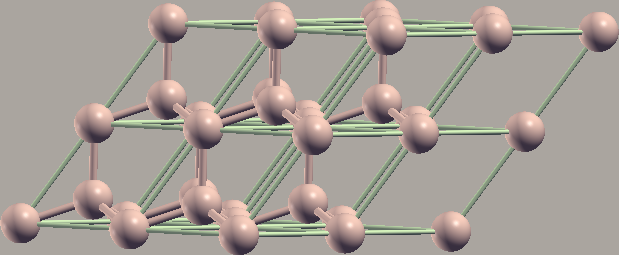
\includegraphics[width=14cm]{../pictures/fcc-Si.png}
\end{center}
%%%%%%%%%%%%%%%%%%%%%%%%%%%%%%%%%%%%%%%%%%%%%%%%%%%%%%%%%%%%%%%%%%%%%%%%%%%%%%%%%%%%%%%%%%%%%%%%%%%% 
\head{Input of \prog{ph.x}}
\parbox{17cm}{
	\begin{itemize}
	\item \prog{ph.x} is quite simple with only one namelist \var{\&inputph}
	\item \var{prefix} and \var{tmp} must match those used by \prog{pw.x} for the scf calculation. 
	\item \var{tr2\_ph} defines the convergence threshold for the self consistent solution of the Sternheimer equations. 
	\item \var{epsilon} asks the program to compute the Electric Field perturbation as well 
	\item \var{fildyn} defines the prefix for the files where the dynamical matrices are saved 
	\item After the namelist we indicate the coordinates of the wavevector for which we want compute the dynamical matrix. 
	\end{itemize}
}
\hskip 2cm
\parbox{8cm}{
\card{
    Phonons at Gamma \\
    \&inputph  \\
     prefix = 'Si'\, \\
     tr2\_ph = 1.0d-14, \\
     amass(1) = 28.0855, \\
     epsil = .true. \\
     outdir = './tmp' \\
     fildyn = 'Si.dyn', \\
    / \\
   0.0  0.0  0.0}
}



%%%%%%%%%%%%%%%%%%%%%%%%%%%%%%%%%%%%%%%%%%%%%%%%%%%%%%%%%%%%%%%%%%%%%%%%%%%%%%%%%%%%
\head{1. How to calculate and plot molecular orbitals}
\rightfooter{Example: \file{Day-1/example1.benzene/}}

To plot signed molecular-orbital densities
($\sign(\psi_i(\vr))|\psi_i(\vr)|^2$), we need to:
\begin{itemize}
\item calculate Kohn-Sham states with \prog{pw.x} (i.e. make an
  SCF calculation)
\item instruct \prog{pp.x} to write them in a suitable format to
  specified files
\item plot orbitals with \prog{xcrysden}
\end{itemize}
See \file{README.md} for detailed instructions.
\vspace{-4cm}
\begin{flushright}
  \includegraphics[width=10cm]{figs/psi2-benzene.png}  
\end{flushright}

%%%%%%%%%%%%%%%%%%%%%%%%%%%%%%%%%%%%%%%%%%%%%%%%%%%%%%%%%%%%% 
\head{1. How to plot molecular orbitals with xcrysden}
\rightfooter{Example: \file{Day-1/example1.benzene/}}

\vspace{-0.5em}
\begin{itemize}
\item Execute in the terminal:\\[0.5em]
  %
  \exec{pw.x < pw.benzene.scf.in > pw.benzene.scf.out}\\
  \exec{pp.x < pp.benzene.scf.in > pp.benzene.scf.out}\\[0.5em]
  % 
  {\small The resulting molecular orbitals (i.e., $\sign(\psi(\vr))|\psi(\vr)|^2$) are
  written to \file{psi2.benzene\_*.xsf}}

  \vspace{-0.5em}
\item Plot one of the generated XSF files with \prog{xcrysden},
  e.g.:\\[0.5em]
  % 
  \exec{xcrysden --xsf psi2.benzene\_K001\_B006.xsf}\\[0.5em]
  %
  and follow these instructions:
  \vspace{-0.5em}
  {\small
    \begin{itemize}
    \item use the menu \file{Tools-->Data Grid}; a new window opens, press \file{[OK]}
    \item an isosurface-control window appear; specify the \file{Isovalue},
      say \file{0.005} and press \file{[Submit]}
    \item click the \file{Render +/- isovalue} radiobutton and again
      press \file{[Submit]}
    \item rotate and zoom the structure according to your preference
    \item save the displayed {\em state} via the menu
      \file{File-->Save Current State}\\
      (e.g., save to \file{my-display.xcrysden})
    \item try this with other orbitals, e.g.:\\[0.3em]
      {\small \exec{xcrysden --xsf psi2.benzene\_K001\_B005.xsf --script
          my-display.xcrysden}}
    \end{itemize}
  }
  \vspace{-0.5em}
\item To plot all orbitals, execute: ~\code{./plot-psi2.sh}
\end{itemize}


%%%%%%%%%%%%%%%%%%%%%%%%%%%%%%%%%%%%%%%%%%%%%%%%%%%%%%%%%%%%%
\head{2. How to calculate a 2D-periodic system: graphene}
\rightfooter{Example: \file{Day-1/example2.graphene/}}
%
\parbox{17cm}{A 2D-periodic system (e.g., a graphene sheet) is
  modelled by adding a vacuum layer in the 3rd direction.\\[-0.5em]

  $\bullet$ move to \file{Day-1/example2.graphene/} directory\\[-0.5em]
  
  $\bullet$ look at the input file \file{pw.graphene.scf.in};
  graphene has a 2-atom hexagonal unit cell in the $xy$ plane:
  \var{ibrav=4}, \var{celldm(1)=4.654},\\
  \var{celldm(3)=}\textit{some suitably large value, e.g.} \var{3.0};
}
\hfill \parbox{8cm}{
  \includegraphics[width=8cm]{figs/graphene.png}\\
}

{\small (remember: \var{celldm(1)} in Bohr radii, \var{celldm(3)=c/a};
  alternatively: \var{A=2.463}, \var{C=7.388} in \AA)}

\parbox{12cm}{
  $\bullet$  atomic positions:\\
\card{
ATOMIC\_POSITIONS (alat)\\
C    0.000000    0.000000    0.000000\\
C    0.000000    0.5773503   0.000000}
}
\hskip 2cm
\parbox{12cm}{
  or, equivalently:\\
  \card{
    ATOMIC\_POSITIONS (crystal)\\
    C    0.000000    0.000000   0.000000\\
    C    0.333333    0.666667   0.000000}
}\\

$\bullet$ k-points: use a dense grid in the $xy$ plane only, e.g.\\
\card{
K\_POINTS (automatic)\\
9 9 1 0 0 0}\\
(a uniform 9$\times$9$\times$1 grid, centered on ${\bf k}=(0,0,0)$ )

%$\bullet$ instructions for how to run the example are in \file{README.md}

%%%%%%%%%%%%%%%%%%%%%%%%%%%%%%%%%%%%%%%%%%%%%%%%%%%%%%%%%%%%%
\head{2. Graphene: DOS and bands (spaghetti)}

\begin{itemize}
\item DOS is typically calculated by a \prog{pw.x} SCF calculation
  followed by a \prog{pw.x} non-SCF calculation (\var{calculation =
    'nscf'}) with a denser k-point grid, and finally using
  \prog{dos.x} post-processing code.

\item to calculate the bands (spaghetti plot), the \prog{pw.x} SCF
  calculation is followed by a \prog{pw.x} ``bands''-type non-SCF
  calculation (\var{calculation = 'bands'}), for which we need a
  suitable path of k-points. The most difficult (?) part is to figure
  out a suitable path of k-points.

  You may either use the ``k-path selection'' tool of \prog{xcrysden}
  or the \prog{SeeK-path} web site at
  \file{http://materialscloud.org/tools/seekpath}.

\item instructions for how to calculate DOS and bands are in \file{README.md}
\end{itemize}

%%%%%%%%%%%%%%%%%%%%%%%%%%%%%%%%%%%%%%%%%%%%%%%%%%%%%%%%%%%%%
\head{K-path selection tool of xcrysden}
~\\[-1.5em]
\centerline{\includegraphics[width=25cm]{figs/xc-k-path.png}}
{\small ({\bf important:} to save k-path in Quantum ESPRESSO format, explicitly
specify the \file{*.pwscf} extension)}

%%%%%%%%%%%%%%%%%%%%%%%%%%%%%%%%%%%%%%%%%%%%%%%%%%%%%%%%%%%%%
\head{SeeK-path @ http://materialscloud.org/tools/seekpath}
~\\
\centerline{\includegraphics[width=24cm]{figs/seekpath.pdf}}
\end{document}

%%% Local Variables:
%%% mode: latex
%%% TeX-master: t
%%% End:
